\section{Introduzione alla gestione aziendale}
\subsection{Gestione d'impresa e attività decisionale}


\begin{itemize}
    \item L'impresa è un sistema socio tecnico aperto
    \item gli obiettivi vengono perseguiti con l'attività decisionale(migliorare produzione e soddisfazione cliente)
\end{itemize}

\begin{figure}[H]
    \centering
    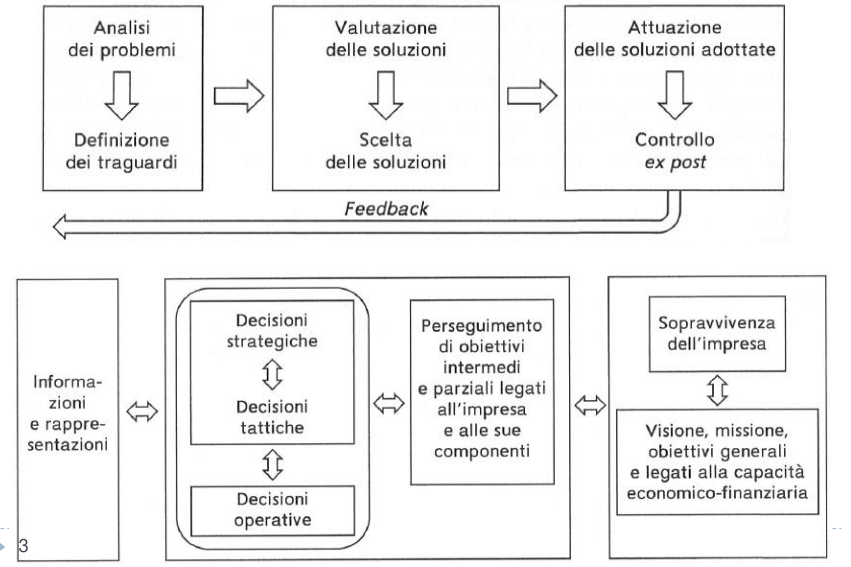
\includegraphics[width=0.7\linewidth]{1/img/Screenshot from 2022-07-03 11-30-16.png}
\end{figure}

\subsection{Criteri di scelta nelle decisioni d'impresa}


3 criteri:
\begin{itemize}
    \item efficacia: scelta e realizzazione degli obbiettivi
    \item efficienza: minimizzare le risorse
        \begin{itemize}
            \item produttività: effcienza tecnica
            \item economicità: effcienza economica
        \end{itemize}
    \item redditività
\end{itemize}

\begin{figure}[H]
    \centering
    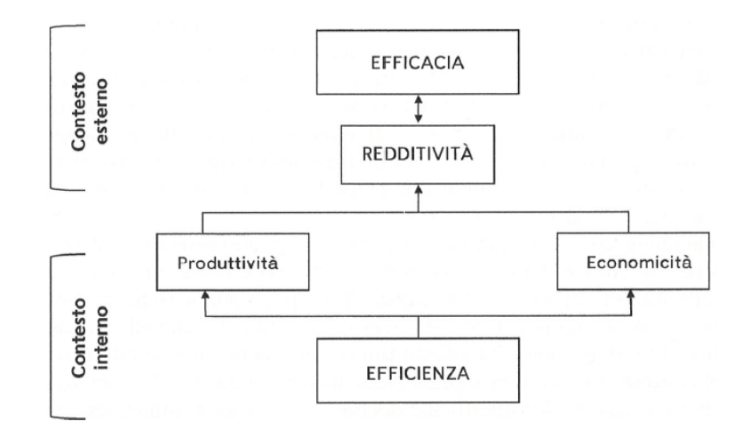
\includegraphics[width=0.5\linewidth]{1/img/Screenshot from 2022-07-03 11-35-16.png}
\end{figure}

\subsection{Incertezza e ambiguità nelle decisioni d'impresa}

\begin{figure}[H]
    \centering
    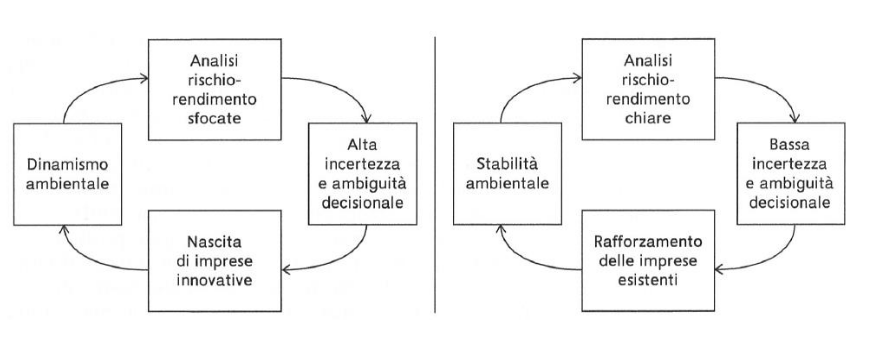
\includegraphics[width=0.7\linewidth]{1/img/Screenshot from 2022-07-03 11-36-56.png}
\end{figure}

\subsection{Le aree funzionali di gestione}

